\section{Context}\label{context}

Biogeographers have long been fascinated by the picture of species
distributions and questioned how it could have been made, i.e.~searching
for the processes shaping biodiversity on Earth ({\textbf{???}},
({\textbf{???}})). Starting from the clear relationship between abiotic
variables and the physiological constraints of organisms, large-scale
studies have been conducted in a pattern-driven perspective making
Biogeography a realm of correlations ({\textbf{???}}). Such an approach
has provided many valuable knowledge along with the development of
efficient statistical tools. However, in the context of global changes,
many researchers claim for strengthening the theoretical foundations of
the field towards a Biogeography mechanism-driven providing reliable
biodiversity forecasts ({\textbf{???}}, ({\textbf{???}}),
({\textbf{???}})).

The importance of biotic constraints on species distribution are one of
the many concerns regarding this request ({\textbf{???}}, Araújo and
Rozenfeld (2014)). In order to test whether interactions influence
species distributions, the simplest avenue is to investigate the species
co-distribution in light of their ecological relationships. Such
investigation started with Diamond's original study stating that species
interacting by competition should avoid each other in space, leading to
a `checkerboard' distribution (Diamond, 1975). This idea was rapidly
criticized for the lack of an adequate null hypothesis ({\textbf{???}},
({\textbf{???}})). Nevertheless, the resulting debate captured the
attention of biogeographers as it must unravel whether co-occurrence
data are more than the sum of occurrence information ({\textbf{???}}).
The answer to this question as direct and major consequences: a negative
one would support the use of classical species distribution models
(hereafter SDMs, ({\textbf{???}})) whereas a positive one would give
credit to methods taking co-occurrence information as a proxy for
ecological interactions ({\textbf{???}}) and would support the
development of methods including network into species distribution
models ({\textbf{???}}, ({\textbf{???}})).

Recent theoretical developments have proposed mechanisms explaining how
ecological interactions must affect the fundamental niche (see Box 1)
and how they could impact occurrence data ({\textbf{???}}, Araújo and
Rozenfeld (2014)). However, ranges of species are very often inferred
from the realized niche which includes the impact of abiotic and biotic
factors. Therefore, finding evidences of interaction signals may prove
difficult which could explain the scarcity of studies reporting such
effect (but see ({\textbf{???}})). Fortunately, the co-occurrence theory
in interaction networks has been formalized and suggests that the
repercussion of interactions in co-occurrence data depends on the
structure of the network ({\textbf{???}}). Notably, the higher the
degree of a species, \emph{i.e} the number of species which with it
interacts, the harder it becomes to link a co-occurrence to an
ecological relationship rather than to a random co-occurrence. Finding
such relationship in empirical data would support the idea that
interactions shape geographic ranges even if for many pairs of
interacting species, no significant co-occurrences are found.

Here, we examined occurrence data in the light of these recent
theoretical developments for five different datasets for which
interactions are observed or assessed to determine whether ecological
interactions impact the distribution of species. We report that the
analysis of co-occurrence failed to clearly reveal a difference between
pairs of interacting species and pairs of not-interacting species.
However our results suggest that the degree of species influences our
ability to detect significant association making co-occurrence
information more than a collection of co-occurrence only for species
with a limited number of link. Moreover we discover a clear relationship
between the co-occurrence strength of a species and the cumulated
occupancy of the entire set of species with which a species interact.
Interestingly, we point out that the relation vanishes when we used
classical SDMs. This results questions the capacity reliability of SDM
for forecasting relevant assemblage of species and support the need for
integrating ecological information into SDMs ({\textbf{???}}).

\section{Material and Methods}\label{material-and-methods}

\subsection{Datasets}\label{datasets}

We analyzed five datasets spawning a large range of environmental
conditions (see Fig S1 and SI Text), a large diversity of organisms and
covering all fundamental type of interactions (see ({\textbf{???}})).
Four of them came with observed interactions based on which we derived
metawebs and computed the connectance associated, the degree of species
and the shortest-path between all pairs of species (see SI Text). For
the North American Trees datasets, we derive a distance based on
functional traits (see table S1 and Fig S2). For the French Breeding
Birds Survey, we also derived different trait-based distance (see table
S2). For all datasets, we kept only species that were present at least
on 1\% of the total number of sites (see SI Text).

\subsection{Measures of co-occurrence}\label{measures-of-co-occurrence}

For each pair of species, we determined the number of observed
co-occurrence \(O_{i,j}\) and we calculated the expected co-occurrence
values \(E_{i,j}\) and its standard deviation \(SD_{i,j}\) to compute a
Z-score \(O_{i,j}-E_{i,j}/SD_{i,j}\) ({\textbf{???}}) whose positive
(negative) values indicates more (less) co-occurrence than randomly
expected. Expectations were derived using three different methods.
First, we assumed that all sites were equivalent, meaning we occulted
the potential influence of abiotic conditions. The distribution of
co-occurrence for a limited number of sites have been already studied
elsewhere ({\textbf{???}}, ({\textbf{???}})), therefore, we used an
hypergeometric distribution (see SI Text for further details). For the
two other expected values, we used two different classical SDMs, namely,
Generalized Linear Model (hereafter GLM) and Radom Forest (hereafter RF)
in order to assign a probability of being presence in a given site for
all species (see SI Text for more details and Fig S3 for the assessment
of performances of the models). Hence, we integrate the possibility that
species may often co-occur simply because they have similar abiotic
requirements.

\section{Results}\label{results}

For two out of four datasets for which interactions were known, we
obtained a difference between interacting and not-interacting species
(\ref{fig:synth} panels A to D). Therefore, when integrating all pairs
of species we did not obtain a clear evidence that interacting species
co-occur differently from not-interacting one. For the willows leafs
network, distinguishing herbivore-willow interactions from
herbivore-parasitoids revealed that the strength of co-occurrence was
stronger for the former interactions than the latter ones
(\ref{fig:shtpth} A-B). Interestingly, we noticed that the higher the
mean degree of species in the dataset, the more difficult the detection
of a signal of interactions in co-occurrence was (\ref{fig:shtpth} A-D).

For the two datasets for which we inferred a distance based on
functional traits, we found that co-occurrence where higher for pairs of
similar species (\ref{fig:synth} panels E and F). As similarity could be
taken as a proxy for competition strength ({\textbf{???}}), this result
suggests that competition is poorly detectable at large scale which is
theoretically supported (Araújo and Rozenfeld, 2014). Therefore,
co-occurrences of similar species are likely driven by the similarity of
their abiotic requirements. The results for the FBBS dataset were
identical irrespective the type of traits examined (Fig S4). This
hypothesis was further supported by the decrease of the Z-score with the
distance for both datasets (fig S6 A and D).

For all datasets, we report that taking environmental context into
account shrinks the distribution and shift it toward 0
(\ref{fig:synth}). Hence, assuming that sites are not identical for
species due to the abiotic context makes the signal of co-occurrence
decreases and sometimes vanished. In the pitcher dataset, we found that
the signal is even reversed but the quality of the SDM approaches were
low (fig S3 B).

Z-scores quickly tend to 0 when the shortest between the two species in
the pair examined increases irrespective the methods employed to
calculate the expected co-occurrence (\ref{fig:shtpth} A-D).
(\ref{fig:shtpth} A-D). Although this was predicted by the theory
({\textbf{???}}), the decay observed is steeper. Therefore the imprint
of indirect interaction in static co-occurrence data sounds
unappreciable. From a prediction perspective, this results suggests that
if species are separated by more than two links, they can be considered
statistically independent. The decay was valid when we all pairs pf
species were examined (see Fig S5).

When abiotic context is not taken into account, we showed that the mean
Z-score of a predator (pollinator), \emph{i.e} Z-scores averaged over
all the set of its preys (host plants), decreases with the total number
of site covered by its preys (\ref{fig:degocc} panels A, D, G and J).
The associated linear regression outperformed the one using the degree
of the species that has been envisioned by the theory (Fig S7).
Therefore, when a predator feeds on a set of preys that jointly cover a
large part of the geographic range studied, the impact of species
interactions is undetectable, but when the joint repartition of the prey
is restricted, the imprint of interactions remains appreciable.
Additionally, we show this relation asymmetric: the decay is less
convincing when the the mean Z-scores of the preys are plotted against
the cumulated range of their predators (fig S8). Hence the imprints of
interactions in static occurrence are appreciated once relevant pair of
specials species are student. When species are highly linked with other
species and when these species have ranges that do not completely
overlap, we cannot make clearly co-occurrence to interactions. This
suggest that the range of the set of species should be examined rather
that individual range of prey. Interestingly, we found that using the
presence of the whole set of prey as predictor to assign the presence of
species outperformed GLMs (see Fig S9). When abiotic constrains are
taken into account, the relationship is weakened or even reversed
(\ref{fig:degocc}) meaning the signals of co-occurrence for specialists
are no longer different from the one of generalists. This illustrates
that inferring species distribution from abiotic requirements cannot
reflect meaningful biological properties of the ecological system
studied.

\subsection{Discussion (\textasciitilde{} 4000
char)}\label{discussion-4000-char}

\textbf{to be written}:

\begin{itemize}
\item
  Our results imply :
\item
  the absence of signal at large scale often observed does not mean that
  interaction are unimportant rather absence of evidence for significant
  co-occurrence may be du to the abundance of interaction.
\item
  co-occurrence studies must be conducted in the light of network
  properties. At least spatial knowledge about the system may help
  searching for pattern of occurrence.
\item
  co-occurrence data have an imprint for specialist and must include it.
\item
  Abundance of interaction occult a signal of co-occurrence.
\item
  For specialists, the relative position of two species within an
  ecological network is a valuable source of information that species
  distribution models must integrate to better deal with the assumption
  that species are independent.
\item
  Biological consistency of SDMs must be questioned. What part of
  interaction are actually hidden by SDM approach? JSDM approaches do a
  better job ?
\item
  Using the whole set of species as one to improve predictions?
\item
  Co-occurrence can be used as a proxy interaction ? In very special
  case (in microbiology it is relevant) or with other source of
  informations \emph{e.g} time series get the covariation of ranges that
  must be a richer information.
\item
  Mechanism-based approaches are needed.
\item
  The ongoing mass extinction is a decline of the total number of
  species on Earth but also a strong drop in the number of links. Our
  results highlight that predictions when interactions are abundant may
  be easier than when they are scarcer and dramatically changed. Hence
  many of the current forecast may prove wrong.
\end{itemize}

\newpage

\subsection{Box 1}\label{box-1}

The fundamental niche is here described as the occurrence probability
under the assumptions that (1) biotic factors are not limiting occupancy
and (2) that dispersion is unconstrained. In this case, only abiotic
factors (such as water availability, temperature variability and edaphic
variables) limits survival and/or reproduction success, and then the
occurrence probability. Consequently, predators occupancy is computed
assuming that preys are abundant enough all along the environmental
gradient. Similarly, the fundamental niche of any prey is not influenced
neither by predators nor by competitors.

For a three species network made of one predator and its two preys, we
derive the three fundamental niches \(f_i\) (\ref{fig:box1} A).
Regarding the predator (species 3), we assume its prey are equivalent
and that the presence of at least one prey is sufficient to release all
the biological constraints:

\[f_3(w)=P(X_3=1|X_2+X_1>0, G=w)\]

where \(G\) denotes the environmental gradient and \(X_i\) is the random
variable associated to the presence of species \(i\). Similarly, \(f_1\)
and \(f_2\) are obtained assuming that 3 is absent :

\[f_2(w)=P(X_2=1|X_3=0, G=w)\]

and:

\[f_1(w)=P(X_1=1|X_3=0, G=w)\]

Once projected on a map, the fundamental niche unravels the potential
distribution of a species ({\textbf{???}}). The expected distribution
can be compared to real observations and could reveal whether dispersal
limits and ecological interactions are prevalent in the occupancy
dynamic of studied species. The realized niche (\ref{fig:box1} B)
includes these factors.\\
In our simplified example, fundamental and realized niches of preys are
identical. The realized niche of the predator, \(r_3\), is controlled by
the joint realized niches of its preys:

\[r_3(w)=f_3(w)\left(1-(1-r_1(w))(1-r_2(w))\right)\]

The above expression may often be more complicated due to the size and
the structure of the network. For instance, we do not consider the
apparent competition between 1 and 2 although it must affect the
distribution of all species. Integrating the impact of many interactions
may be possible using occurrence probabilities of species assemblages
rather than single species ({\textbf{???}}). Integrating network
information to shed light upon species distribution is also crucial to
understand what kind of co-occurrence is biologically relevant. Consider
as an example the co-occurrence between species 1 and 3: the
co-occurrence may be strong if we restrict the analysis to the suitable
conditions for species 1 but it must be weak if the entire environmental
gradient is sampled. However, if we examine the co-occurrence between 3
and the assemblage made of species 1 plus 2, the co-occurrence may
always be strong. Although this is meaningful in a biological point of
view, co-occurrence studies often remain focus on pairs of species.

\newpage

\subsection{Tables}\label{tables}

\begin{longtable}[]{@{}lrrrrrrr@{}}
\caption{Data sets analyzed in this article.
\label{tbl:data}}\tabularnewline
\toprule
\begin{minipage}[b]{0.15\columnwidth}\raggedright\strut
Type\strut
\end{minipage} & \begin{minipage}[b]{0.07\columnwidth}\raggedleft\strut
No. of sites\strut
\end{minipage} & \begin{minipage}[b]{0.07\columnwidth}\raggedleft\strut
No. of species\strut
\end{minipage} & \begin{minipage}[b]{0.11\columnwidth}\raggedleft\strut
Interaction type\strut
\end{minipage} & \begin{minipage}[b]{0.05\columnwidth}\raggedleft\strut
Observed\strut
\end{minipage} & \begin{minipage}[b]{0.04\columnwidth}\raggedleft\strut
Traits\strut
\end{minipage} & \begin{minipage}[b]{0.06\columnwidth}\raggedleft\strut
Connectance\strut
\end{minipage} & \begin{minipage}[b]{0.22\columnwidth}\raggedleft\strut
References\strut
\end{minipage}\tabularnewline
\midrule
\endfirsthead
\toprule
\begin{minipage}[b]{0.15\columnwidth}\raggedright\strut
Type\strut
\end{minipage} & \begin{minipage}[b]{0.07\columnwidth}\raggedleft\strut
No. of sites\strut
\end{minipage} & \begin{minipage}[b]{0.07\columnwidth}\raggedleft\strut
No. of species\strut
\end{minipage} & \begin{minipage}[b]{0.11\columnwidth}\raggedleft\strut
Interaction type\strut
\end{minipage} & \begin{minipage}[b]{0.05\columnwidth}\raggedleft\strut
Observed\strut
\end{minipage} & \begin{minipage}[b]{0.04\columnwidth}\raggedleft\strut
Traits\strut
\end{minipage} & \begin{minipage}[b]{0.06\columnwidth}\raggedleft\strut
Connectance\strut
\end{minipage} & \begin{minipage}[b]{0.22\columnwidth}\raggedleft\strut
References\strut
\end{minipage}\tabularnewline
\midrule
\endhead
\begin{minipage}[t]{0.15\columnwidth}\raggedright\strut
Willow Leaf Network\strut
\end{minipage} & \begin{minipage}[t]{0.07\columnwidth}\raggedleft\strut
374\strut
\end{minipage} & \begin{minipage}[t]{0.07\columnwidth}\raggedleft\strut
156\strut
\end{minipage} & \begin{minipage}[t]{0.11\columnwidth}\raggedleft\strut
Trophic / Parasitism\strut
\end{minipage} & \begin{minipage}[t]{0.05\columnwidth}\raggedleft\strut
yes\strut
\end{minipage} & \begin{minipage}[t]{0.04\columnwidth}\raggedleft\strut
no\strut
\end{minipage} & \begin{minipage}[t]{0.06\columnwidth}\raggedleft\strut
0.042\strut
\end{minipage} & \begin{minipage}[t]{0.22\columnwidth}\raggedleft\strut
unpublished\strut
\end{minipage}\tabularnewline
\begin{minipage}[t]{0.15\columnwidth}\raggedright\strut
Pitcher Plants Network\strut
\end{minipage} & \begin{minipage}[t]{0.07\columnwidth}\raggedleft\strut
39x20\strut
\end{minipage} & \begin{minipage}[t]{0.07\columnwidth}\raggedleft\strut
53\strut
\end{minipage} & \begin{minipage}[t]{0.11\columnwidth}\raggedleft\strut
Trophic\strut
\end{minipage} & \begin{minipage}[t]{0.05\columnwidth}\raggedleft\strut
yes\strut
\end{minipage} & \begin{minipage}[t]{0.04\columnwidth}\raggedleft\strut
no\strut
\end{minipage} & \begin{minipage}[t]{0.06\columnwidth}\raggedleft\strut
0.44\strut
\end{minipage} & \begin{minipage}[t]{0.22\columnwidth}\raggedleft\strut
({\textbf{???}})\strut
\end{minipage}\tabularnewline
\begin{minipage}[t]{0.15\columnwidth}\raggedright\strut
Caribbean Hummingbirds Network\strut
\end{minipage} & \begin{minipage}[t]{0.07\columnwidth}\raggedleft\strut
32\strut
\end{minipage} & \begin{minipage}[t]{0.07\columnwidth}\raggedleft\strut
62\strut
\end{minipage} & \begin{minipage}[t]{0.11\columnwidth}\raggedleft\strut
Mutualist\strut
\end{minipage} & \begin{minipage}[t]{0.05\columnwidth}\raggedleft\strut
yes\strut
\end{minipage} & \begin{minipage}[t]{0.04\columnwidth}\raggedleft\strut
no\strut
\end{minipage} & \begin{minipage}[t]{0.06\columnwidth}\raggedleft\strut
0.011\strut
\end{minipage} & \begin{minipage}[t]{0.22\columnwidth}\raggedleft\strut
({\textbf{???}}), ({\textbf{???}}), ({\textbf{???}})\strut
\end{minipage}\tabularnewline
\begin{minipage}[t]{0.15\columnwidth}\raggedright\strut
North American Trees\strut
\end{minipage} & \begin{minipage}[t]{0.07\columnwidth}\raggedleft\strut
128891\strut
\end{minipage} & \begin{minipage}[t]{0.07\columnwidth}\raggedleft\strut
31\strut
\end{minipage} & \begin{minipage}[t]{0.11\columnwidth}\raggedleft\strut
Competition\strut
\end{minipage} & \begin{minipage}[t]{0.05\columnwidth}\raggedleft\strut
yes\strut
\end{minipage} & \begin{minipage}[t]{0.04\columnwidth}\raggedleft\strut
no\strut
\end{minipage} & \begin{minipage}[t]{0.06\columnwidth}\raggedleft\strut
-\strut
\end{minipage} & \begin{minipage}[t]{0.22\columnwidth}\raggedleft\strut
unpublished\strut
\end{minipage}\tabularnewline
\begin{minipage}[t]{0.15\columnwidth}\raggedright\strut
French Breeding Birds Survey\strut
\end{minipage} & \begin{minipage}[t]{0.07\columnwidth}\raggedleft\strut
2354\strut
\end{minipage} & \begin{minipage}[t]{0.07\columnwidth}\raggedleft\strut
179\strut
\end{minipage} & \begin{minipage}[t]{0.11\columnwidth}\raggedleft\strut
Trophic\strut
\end{minipage} & \begin{minipage}[t]{0.05\columnwidth}\raggedleft\strut
yes\strut
\end{minipage} & \begin{minipage}[t]{0.04\columnwidth}\raggedleft\strut
no\strut
\end{minipage} & \begin{minipage}[t]{0.06\columnwidth}\raggedleft\strut
0.018\strut
\end{minipage} & \begin{minipage}[t]{0.22\columnwidth}\raggedleft\strut
Gaüzère et al. (2015)\strut
\end{minipage}\tabularnewline
\bottomrule
\end{longtable}

\newpage

\section{Figures}\label{figures}

\begin{figure}[htbp]
\centering
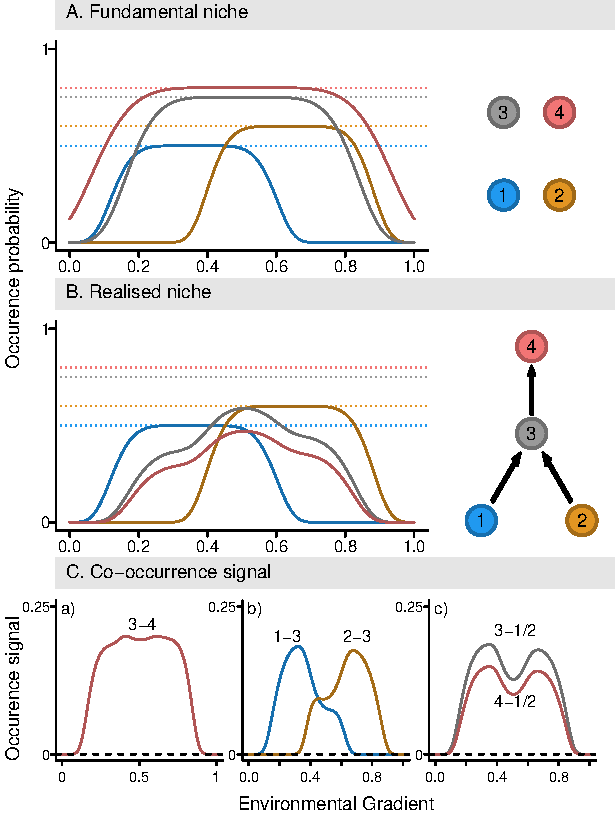
\includegraphics{../fig/figConcept.pdf}
\caption{\textbf{Probabilistic description of fundamental and realized
niches} For a three species network all the occurrence probabilities are
derived along an environmental gradient assuming that A interactions are
not limiting the distribution and B that species 3 needs at least of one
of its preys, \emph{i.e.} species 1 or 2. Horizontal dotted lines stand
for the occurrence probabilities reached at an environmental
optimum.\label{fig:box1}}
\end{figure}

\newpage

\begin{figure}[htbp]
\centering
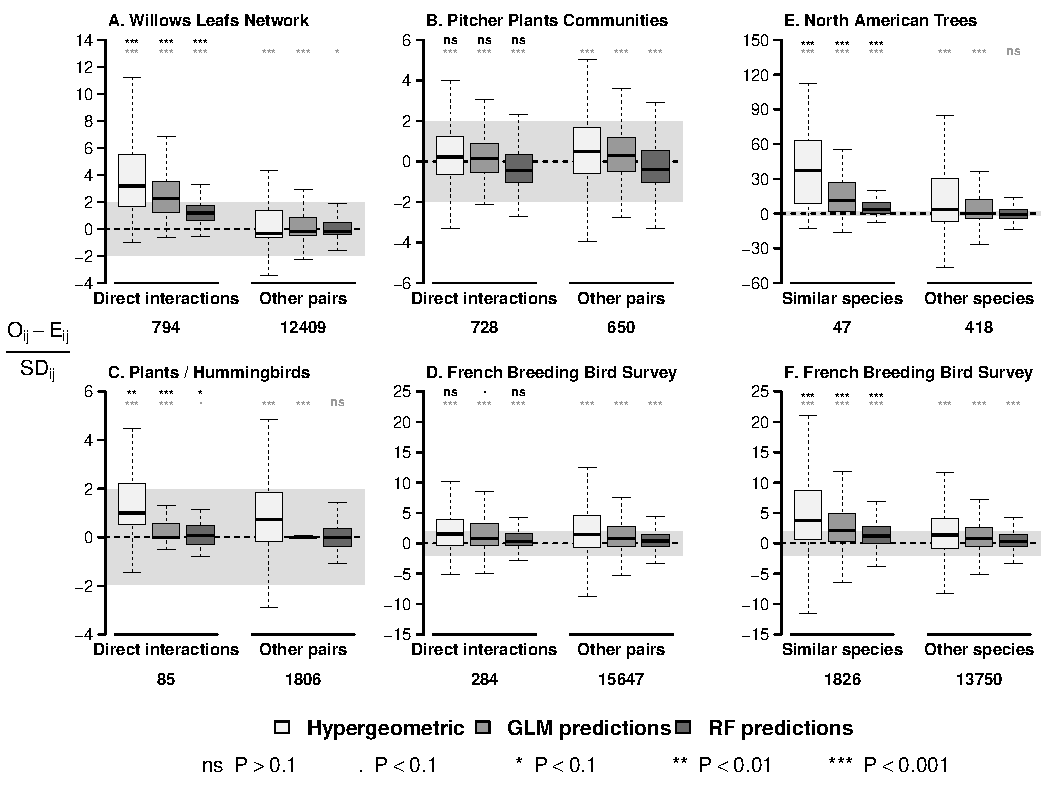
\includegraphics{../fig/figIntVsNoint.pdf}
\caption{\textbf{Co-occurrence of interacting versus not-interacting
pairs of species} Figures under each groups of boxplots indicate the
number of pairs to which the Z-score distributions refer. The light grey
rectangle corresponds to the 95\% confidence interval for the standard
normal distribution which gives insight into the proportion of pairs of
species significantly different from 0. The comparison made in panels A
to D is based on direct interactions observed. For panels E and F,
similar species are defined as the species for which the trait-based
distance is less than or equal to the lower decile of this distance
distribution. Note that outliers are not displayed. P values were
computed using the Wilcoxon rank sum test, to compare interacting versus
not-interacting Z-score distribution calculated for the three different
methods (black symbols) and to show whether the distribution is
symmetric about 0.\label{fig:synth}}
\end{figure}

\newpage

\begin{figure}[htbp]
\centering
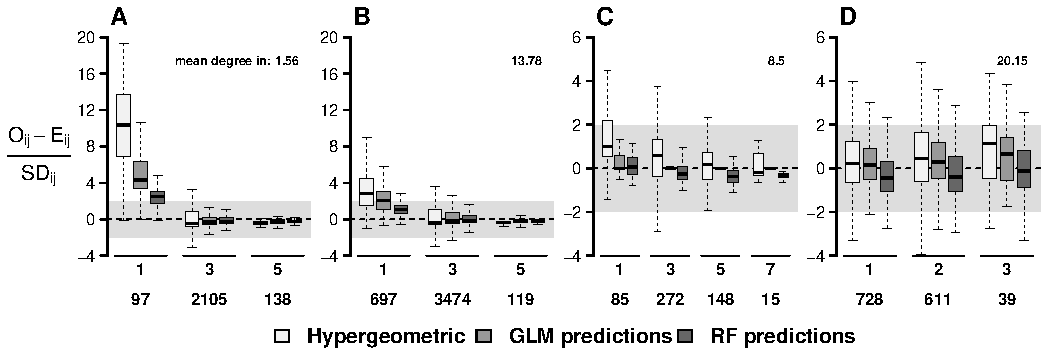
\includegraphics{../fig/figOrder.pdf}
\caption{\textbf{Co-occurrence signal decays when the shortest path
between a pair of species decay } The Z-score distribution are plotted
against the shortest path for A willows-herbivores interactions, B
herbivores-parasitoids interactions, C birds-plants interactions and D
the pitcher plants network. First figures under each grouped boxplots
indicate the shortest path associated while the figures below provide
the number of pair to which the distribution refers.\label{fig:shtpth}}
\end{figure}

\newpage

\begin{figure}[htbp]
\centering
\includegraphics{../fig/figdegocc.pdf}
\caption{\textbf{Co-occurrence significance decreases as the cumulated
occupancy increases} For a given species, Z-scores are averaged over the
all set species it interacts with and plotted against the joint
distribution of the same set of species. We do so for the herbivores in
the willows leafs network (panels A to C), the parasitoids in the willow
leafs network (panels D to F), the hummingbirds in the Caribbean
hummingbirds datasets (panels G to I) and all species in the pitcher
plants network that consume other species (panels J to L). The x-axis is
expressed as a log proportion of the total number of sites. Black
symbols are mean Z-scores significantly different from 0 (see SI Text).
In each panel, the dotted line represents the linear regression
\(y~ax+b\) for which the \(R^2\) is provided. The size of circles
reflects the degree of species for which the Z-score was calculated, the
relation size-degree for each row is given in the middle panel. For the
hummingbirds dataset (panels G to I), the triangle represent the values
obtained for the former distribution of a species already analyzed (see
SI text).\label{fig:degocc}}
\end{figure}

\newpage

\section*{Reference}\label{reference}
\addcontentsline{toc}{section}{Reference}

\hypertarget{refs}{}
\hypertarget{ref-Araujo2014}{}
Araújo, M.B., Rozenfeld, A., 2014. The geographic scaling of biotic
interactions. Ecography 37, 406--415.
doi:\href{https://doi.org/10.1111/j.1600-0587.2013.00643.x}{10.1111/j.1600-0587.2013.00643.x}

\hypertarget{ref-Diamond1975}{}
Diamond, J.M., 1975. Assembly of species communities, in: Cody, M.L.,
Diamond, J.M. (Eds.), Ecology and Evolution of Communities. Harvard
University Press, Cambridge, Massachusetts, USA., pp. 342--444.

\hypertarget{ref-Gauzere2015}{}
Gaüzère, P., Jiguet, F., Devictor, V., 2015. Rapid adjustment of bird
community compositions to local climatic variations and its functional
consequences. Global Change Biology n/a--n/a.
doi:\href{https://doi.org/10.1111/gcb.12917}{10.1111/gcb.12917}
\section{Material and methods}\label{material-and-methods}

In this section, we present in more details, the datasets and the
methodology we used. All analyses have been performed using R
environment software (table S1 includes functions and packages we used).

\subsection{Datasets}\label{datasets}

Sites for the five datasets are reported on five maps gathered in Fig
S1. Below, we describe in more details the five datasets. The total
number of species, the number of species present in at least 1\% of the
total number of site and the number of species for which traits
information were available are reported in table S2.

\subsubsection{Willows leafs network}\label{willows-leafs-network}

\subsubsection{Pitcher plants network}\label{pitcher-plants-network}

\subsubsection{Caribbean Hummingbirds-Plant
network}\label{caribbean-hummingbirds-plant-network}

\subsubsection{North American Trees
datasets}\label{north-american-trees-datasets}

\paragraph{Traits-based distance}\label{traits-based-distance}

We used a distance built upon nine functional traits whose values were
retrieved from ({\textbf{???}}), see \textbf{Supplementary Table 3}
available at
\url{http://onlinelibrary.wiley.com/doi/10.1111/j.1466-8238.2010.00592.x/suppinfo}.
Each of the nine selected variables were centered and scaled (R
functions used reported in table S1) then used as is to derive Euclidean
distances for all pairs of species. Then, we use agglomeration
clustering with Ward's method (implemented in the \emph{hclust()}
function we used, see Table S1) to obtain the dendrogram presented in
\ref{fig:dendro}.

\subsubsection{French Breeding Birds Survey
datasets}\label{french-breeding-birds-survey-datasets}

\paragraph{Traits-based distance}\label{traits-based-distance-1}

We used 73 traits that are boolean variable (see Table S4) we kept as is
to derive Euclidean distances for all pairs of species.

\subsection{Building metawebs}\label{building-metawebs}

For four datasets, we built network based on all observed interactions
and derived associated quantities, \emph{i.e.} the connectance of the
metawebs, the degrees of species and the shortest-path, using the R
package ``igraph'' (table S1).

\subsection{Co-occurrence measurement}\label{co-occurrence-measurement}

For a given pair of species \(i\) and \(j\), we examined the
relationship between the observed co-occurrence \(O_{i,j}\) and the
expected co-occurrence \(E_{i,j}\). Here, we provide more information
about the three methods wed used to analyse co-occurrence.

\subsection{Hypergeometric
distribution}\label{hypergeometric-distribution}

This distribution has been mentioned in a different context (see
{\textbf{???}}) and have been fully exploited in ({\textbf{???}})
despite the author never mentioned it is a classical distribution. To
clarify this, we start from the distribution written in equation (1) in
Veech (2013). We consider the co-occurrence of two species on \(n\)
sites. Species 1 is present in \(n_1\) while species 2 is present in
\(n_2\) sites. The probability of having \(j\) co\_occurrence, \(p_j\)
is:

\[ p_j= \frac{\binom{n}{j} \binom{n-j}{n_2-j} \binom{n-n_2}{n_1-j}}{\binom{n}{n_2} \binom{n}{n_2}} \]

if \(\max{0, n_1+n_2-n} \leq j \leq \min{n_1, n_2}\) and 0 otherwise.
The expression above yields:

\[ p_j= \frac{n!}{(n-j)!j!} \frac{(n-j)!}{(n-j-n_2+j)!(n_2-j)!} \frac{(n-n_2)!}{(n-n_2-n_1+j)!(n_1-j)!} \frac{(n-n_1)!n_1!}{n!} \frac{1}{\binom{n}{n_2}} \]

by rearrangement:

\[ p_j= \frac{1}{j!} \frac{1}{(n_2-j)!} \frac{1}{(n-n_2-n_1+j)!(n_1-j)!} \frac{(n-n_1)!n_1!}{1} \frac{1}{\binom{n}{n_2}} \]

once sorted out, this results in:

\[ p_j= \frac{\binom{n_1}{j} \binom{n-n_1}{n_2-j}}{\binom{n}{n_2}} \]

Thus, the number of co-occurrence follows a hypergeometric distribution
of parameters \((n,n_1,n_2)\) we used to calculated the expected
co-occurrence \(E_{i,j}\) under the hypothesis that all site were
identical for all species.

\subsection{GLM and RF}\label{glm-and-rf}

For GLM and RF, \(E_{i,j}\) correspond to probabilities of occurrence
computed based on climatic data. R functions are reported in Table S1.

\subsubsection{Climatic data}\label{climatic-data}

We used the global climate layers provided data WolrdClim, version 1.4,
available at \url{http://www.worldclim.org} ({\textbf{???}}). For each
dataset, we performed a principal component analysis and keep as many
axes as needed to explain 90\% of the total inertia. We used these axis
in GLM and RF.

\subsubsection{Generalized Linear Model}\label{generalized-linear-model}

For all datasets, we performed a Generalized Linear Model
({\textbf{???}}) using all the axis provided by the PCA as polynomials
of degree 2. To constraints the number of parameters, we did not
evaluate the interactions among axis. We also performed a selection
model based on the Akaike's information criterion (AIC) C in a Stepwise
Algorithm. R functions used to carry out the analyses are indexed in
table SX.

\subsubsection{Random Forests}\label{random-forests}

Random Forests ({\textbf{???}}) were performed using the same formula as
for GLMs. For all species, 10000 trees were computed and the probability
for a species being in a given site were calculated based on the number
of votes the sites were granted.

\subsubsection{Evaluating the models}\label{evaluating-the-models}

For all species, we assess the performance of the Species Distribution
Models we used, \emph{i.e.} Generalized Linear Model and Random Forest,
using the Area Under the Receiver Operating Characteristic (AUROC)
({\textbf{???}}). We present the results as a cumulative sum of
frequencies corresponding to the score for all species for each of the
four ecological systems we studied (see Fig ({\textbf{???}})).

\section{Supporting Tables}\label{supporting-tables}

\subsubsection{R packages used}\label{r-packages-used}

\begin{longtable}[]{@{}lrrrr@{}}
\toprule
Analysis & Function & Package name & Version & Citation\tabularnewline
\midrule
\endhead
Scaling and Centering & scale & base & 3.3.1 & R Core Team
(2015)\tabularnewline
Euclidean distance & dist & stats & 3.3.1 & R Core Team
(2015)\tabularnewline
Clustering & hclust & stats & 3.3.1 & R Core Team (2015)\tabularnewline
PCA & dudi.pca & ade4 & 1.7.4 & Dray and Dufour (2007)\tabularnewline
GLM & glm & stats & 3.3.1 & R Core Team (2015)\tabularnewline
GLM Selection & step & stats & 3.3.1 & R Core Team (2015)\tabularnewline
Degree of species & degree & igraph & 1.0.1 &
({\textbf{???}})\tabularnewline
Shortest Paths & shortest.paths & igraph & 1.0.1 &
({\textbf{???}})\tabularnewline
AUROC & somers2 & Hmisc & 3.17.2 & ({\textbf{???}})\tabularnewline
TSN retrieving & get\_tsn & taxize & 0.7.4 & ({\textbf{???}}),
({\textbf{???}})\tabularnewline
Wilcoxon tests & wilcox.test & stats & 3.3.1 & R Core Team
(2015)\tabularnewline
\bottomrule
\end{longtable}

\textbf{Supplementary Table 1}: R and packages used for the analyses.
GLM: Generalized Linear Model, PCA: Principal Component Analysis. AUROC:
Area Under the Receiver Operating Characteristic.\{\#tbl:code\}

\begin{longtable}[]{@{}lrrr@{}}
\toprule
Type & Total & Selected & Traits\tabularnewline
\midrule
\endhead
Willow Leaf Network & 274 & 156 & - ~\tabularnewline
Pitcher Plants Network & 91 & 53 & -\tabularnewline
Caribbean Hummingbirds Network & 62 & 62 & -\tabularnewline
North American Trees & 31 & 31 & 31\tabularnewline
French Breeding Birds Survey & 340 & 179 & 321\tabularnewline
\bottomrule
\end{longtable}

\textbf{Supplementary Table 2}: For each datasets the total number of
species (column \emph{Total}), the number of species present in more
that 1\% of the total number of sites (column \emph{Selected}), andthe
number of species for which traits information are available (column
\emph{Traits}). The symbol `-' means `not relevant'. \{\#tbl:numsp\}

\begin{longtable}[]{@{}lrrrrrrrrrr@{}}
\toprule
Species & TSN & maxH & GR & WD & TolS & TolD & AM & EM & LMA &
Nmass\tabularnewline
\midrule
\endhead
Abies balsamea & 18032 & 25 & 1 & 0.34 & 5.0 & 1.0 & 0 & 1 & 151.00 &
1.66\tabularnewline
Acer negundo & 28749 & 20 & 3 & 0.44 & 3.5 & 3.0 & 1 & 0 & 37.04 &
2.50\tabularnewline
Acer rubrum & 28728 & 25 & 3 & 0.49 & 3.4 & 1.8 & 1 & 0 & 71.09 &
1.91\tabularnewline
Acer saccharum & 28731 & 35 & 1 & 0.56 & 4.8 & 2.3 & 1 & 0 & 70.63 &
1.83\tabularnewline
Betula alleghaniensis & 19481 & 25 & 3 & 0.55 & 3.2 & 3.0 & 0 & 1 &
46.08 & 2.20\tabularnewline
Betula papyrifera & 19489 & 25 & 3 & 0.48 & 1.5 & 2.0 & 0 & 1 & 77.88 &
2.31\tabularnewline
Carpinus caroliniana & 19504 & 8 & 1 & 0.58 & 4.6 & 2.0 & 0 & 1 & 49.05
& 2.15\tabularnewline
Carya cordiformis & 19227 & 25 & 1 & 0.60 & 2.1 & 4.0 & 0 & 1 & 44.05 &
2.60\tabularnewline
Fagus grandifolia & 19462 & 25 & 1 & 0.56 & 4.8 & 1.5 & 0 & 1 & 61.22 &
2.04\tabularnewline
Fraxinus americana & 32931 & 30 & 2 & 0.55 & 2.5 & 2.4 & 1 & 0 & 76.75 &
2.12\tabularnewline
Fraxinus nigra & 32945 & 20 & 2 & 0.45 & 3.0 & 2.0 & 1 & 0 & 71.94 &
2.10\tabularnewline
Fraxinus pennsylvanica & 32929 & 25 & 3 & 0.53 & 3.1 & 3.9 & 1 & 0 &
87.72 & 1.80\tabularnewline
Larix laricina & 183412 & 25 & 3 & 0.48 & 1.0 & 2.0 & 0 & 1 & 120.00 &
1.36\tabularnewline
Ostrya virginiana & 19511 & 12 & 1 & 0.63 & 4.6 & 3.3 & 1 & 0 & 37.04 &
2.20\tabularnewline
Picea glauca & 183295 & 25 & 1 & 0.35 & 4.2 & 2.9 & 0 & 1 & 302.86 &
1.28\tabularnewline
Picea mariana & 183302 & 20 & 1 & 0.41 & 4.1 & 2.0 & 0 & 1 & 294.12 &
1.12\tabularnewline
Picea rubens & 18034 & 25 & 2 & 0.38 & 4.4 & 2.5 & 0 & 1 & 304.67 &
1.15\tabularnewline
Pinus banksiana & 183319 & 20 & 3 & 0.42 & 1.4 & 4.0 & 0 & 1 & 243.90 &
1.24\tabularnewline
Pinus resinosa & 183375 & 25 & 3 & 0.39 & 1.9 & 3.0 & 0 & 1 & 294.12 &
1.17\tabularnewline
Pinus strobus & 183385 & 30 & 3 & 0.36 & 3.2 & 2.3 & 0 & 1 & 121.92 &
1.42\tabularnewline
Populus balsamifera & 22453 & 25 & 3 & 0.37 & 1.3 & 1.8 & 1 & 1 & 83.46
& 1.95\tabularnewline
Populus grandidentata & 22463 & 20 & 3 & 0.39 & 1.2 & 2.5 & 1 & 1 &
70.45 & 2.50\tabularnewline
Populus tremuloides & 195773 & 25 & 3 & 0.37 & 1.2 & 1.8 & 1 & 1 & 82.02
& 2.16\tabularnewline
Prunus pensylvanica & 24799 & 12 & 3 & 0.36 & 1.0 & 2.0 & 1 & 1 & 50.00
& 2.40\tabularnewline
Quercus alba & 19290 & 35 & 1 & 0.60 & 2.9 & 3.6 & 0 & 1 & 81.21 &
2.39\tabularnewline
Quercus macrocarpa & 19287 & 15 & 1 & 0.58 & 2.7 & 3.9 & 0 & 1 & 92.74 &
2.27\tabularnewline
Quercus rubra & 19408 & 25 & 2 & 0.56 & 2.8 & 2.9 & 0 & 1 & 84.20 &
2.06\tabularnewline
Thuja occidentalis & 505490 & 15 & 1 & 0.30 & 3.5 & 2.7 & 1 & 0 & 223.00
& 1.02\tabularnewline
Tsuga canadensis & 183397 & 30 & 1 & 0.40 & 4.8 & 1.0 & 0 & 1 & 122.55 &
0.99\tabularnewline
Ulmus americana & 19049 & 35 & 3 & 0.46 & 3.1 & 2.9 & 1 & 0 & 79.47 &
2.07\tabularnewline
Ulmus rubra & 19050 & 25 & 3 & 0.48 & 3.3 & 3.0 & 1 & 0 & 59.88 &
2.50\tabularnewline
\bottomrule
\end{longtable}

\textbf{Supplementary Table 3}: Tree species and traits used.
Abbreviations are as follows: TSN - Taxonomic Serial Number defined by
Integrated Taxonomic Information System (ITIS), maxH - Average maximum
height, GR - Growth rate, WD - Wood Density, TolS - Shade tolerance,
TolD - Drought tolerance, AM - Arbuscular mycorrhiza (Endomycorrhiza),
EM - Ectomycorrhiza, LMA - Leaf mass per area, Nmass - Nitrogen content
per leaf mass unit({\textbf{???}}) availale at
\url{http://onlinelibrary.wiley.com/doi/10.1111/j.1466-8238.2010.00592.x/suppinfo}.\{\#tbl:trees\}

\begin{longtable}[]{@{}lr@{}}
\toprule
Category & Trait name\tabularnewline
\midrule
\endhead
Activity & Nocturnal\tabularnewline
Activity & Crepuscular\tabularnewline
Activity & Diurnal\tabularnewline
Diet & Seeds, nuts or grain\tabularnewline
Diet & Fruits / frugivory\tabularnewline
Diet & Vegetative\tabularnewline
Diet & invert\tabularnewline
Diet & fish\tabularnewline
Diet & Very small mammals\tabularnewline
Diet & Large mammals\tabularnewline
Diet & Herptile\tabularnewline
Diet & Small birds\tabularnewline
Diet & Long birds\tabularnewline
Diet & Vertebrate\tabularnewline
Diet & Bones\tabularnewline
Diet & Carrion\tabularnewline
Feeding behavior & Pursuit (air and/or aquatic)\tabularnewline
Feeding behavior & Sally\tabularnewline
Feeding behavior & Foliage gleaning\tabularnewline
Feeding behavior & Pouncing\tabularnewline
Feeding behavior & Grazing\tabularnewline
Feeding behavior & Picking, pecking or stabbing\tabularnewline
Feeding behavior & Digging\tabularnewline
Feeding behavior & Overturning\tabularnewline
Feeding behavior & Probing\tabularnewline
Feeding behavior & Filtering\tabularnewline
Feeding habitat & Water-surface\tabularnewline
Feeding habitat & Underwater\tabularnewline
Feeding habitat & Water\tabularnewline
Feeding habitat & Mud\tabularnewline
Feeding habitat & Ground\tabularnewline
Feeding habitat & Canopy\tabularnewline
Feeding habitat & Shrub (low and high)\tabularnewline
Feeding habitat & Vegetation\tabularnewline
Feeding habitat & Air\tabularnewline
Foraging habitat & Wet grassland, meadows, fens, sedges or
tundra\tabularnewline
Foraging habitat & Dry grassland\tabularnewline
Foraging habitat & Rocky slope\tabularnewline
Foraging habitat & Fast river/stream\tabularnewline
Foraging habitat & Slow river/stream\tabularnewline
Foraging habitat & Shore (marine)\tabularnewline
Foraging habitat & Salt marsh\tabularnewline
Foraging habitat & Mud or silt\tabularnewline
Foraging habitat & Sandy gravel/beach\tabularnewline
Foraging habitat & Reed marshes\tabularnewline
Foraging habitat & Conifer\tabularnewline
Foraging habitat & Mixed forest\tabularnewline
Foraging habitat & Deciduous\tabularnewline
Foraging habitat & Mediterranean oak or other\tabularnewline
Foraging habitat & Open/low forest\tabularnewline
Foraging habitat & Forest or habitat edge\tabularnewline
Foraging habitat & Shrub/bush\tabularnewline
Foraging habitat & Urban\tabularnewline
Foraging habitat & Garden\tabularnewline
Foraging habitat & High air\tabularnewline
Nesting habitat & Wet grassland, meadows, fens, sedges or
tundra\tabularnewline
Nesting habitat & Dry grassland\tabularnewline
Nesting habitat & Banks/sand/mud\tabularnewline
Nesting habitat & Rock surface/outcrops\tabularnewline
Nesting habitat & Near water/shore/island\tabularnewline
Nesting habitat & Sand gravel/beach\tabularnewline
Nesting habitat & Reed marshes\tabularnewline
Nesting habitat & Conifer\tabularnewline
Nesting habitat & Mixed forest\tabularnewline
Nesting habitat & Deciduous\tabularnewline
Nesting habitat & Mediterranean oak and other\tabularnewline
Nesting habitat & Open/low forest\tabularnewline
Nesting habitat & Shrub/bush\tabularnewline
Nesting habitat & Urban\tabularnewline
Nesting habitat & Garden\tabularnewline
Nesting location & Elevated\tabularnewline
Nesting location & Tree hole\tabularnewline
Nesting location & Ground\tabularnewline
\bottomrule
\end{longtable}

\textbf{Supplementary Table 4}: List of the Boolean traits used to
derive Euclidean distances between all pairs of species in the French
Breeding Birds Survey.

\newpage

\section{Supporting Figures}\label{supporting-figures}

\begin{figure}[htbp]
\centering
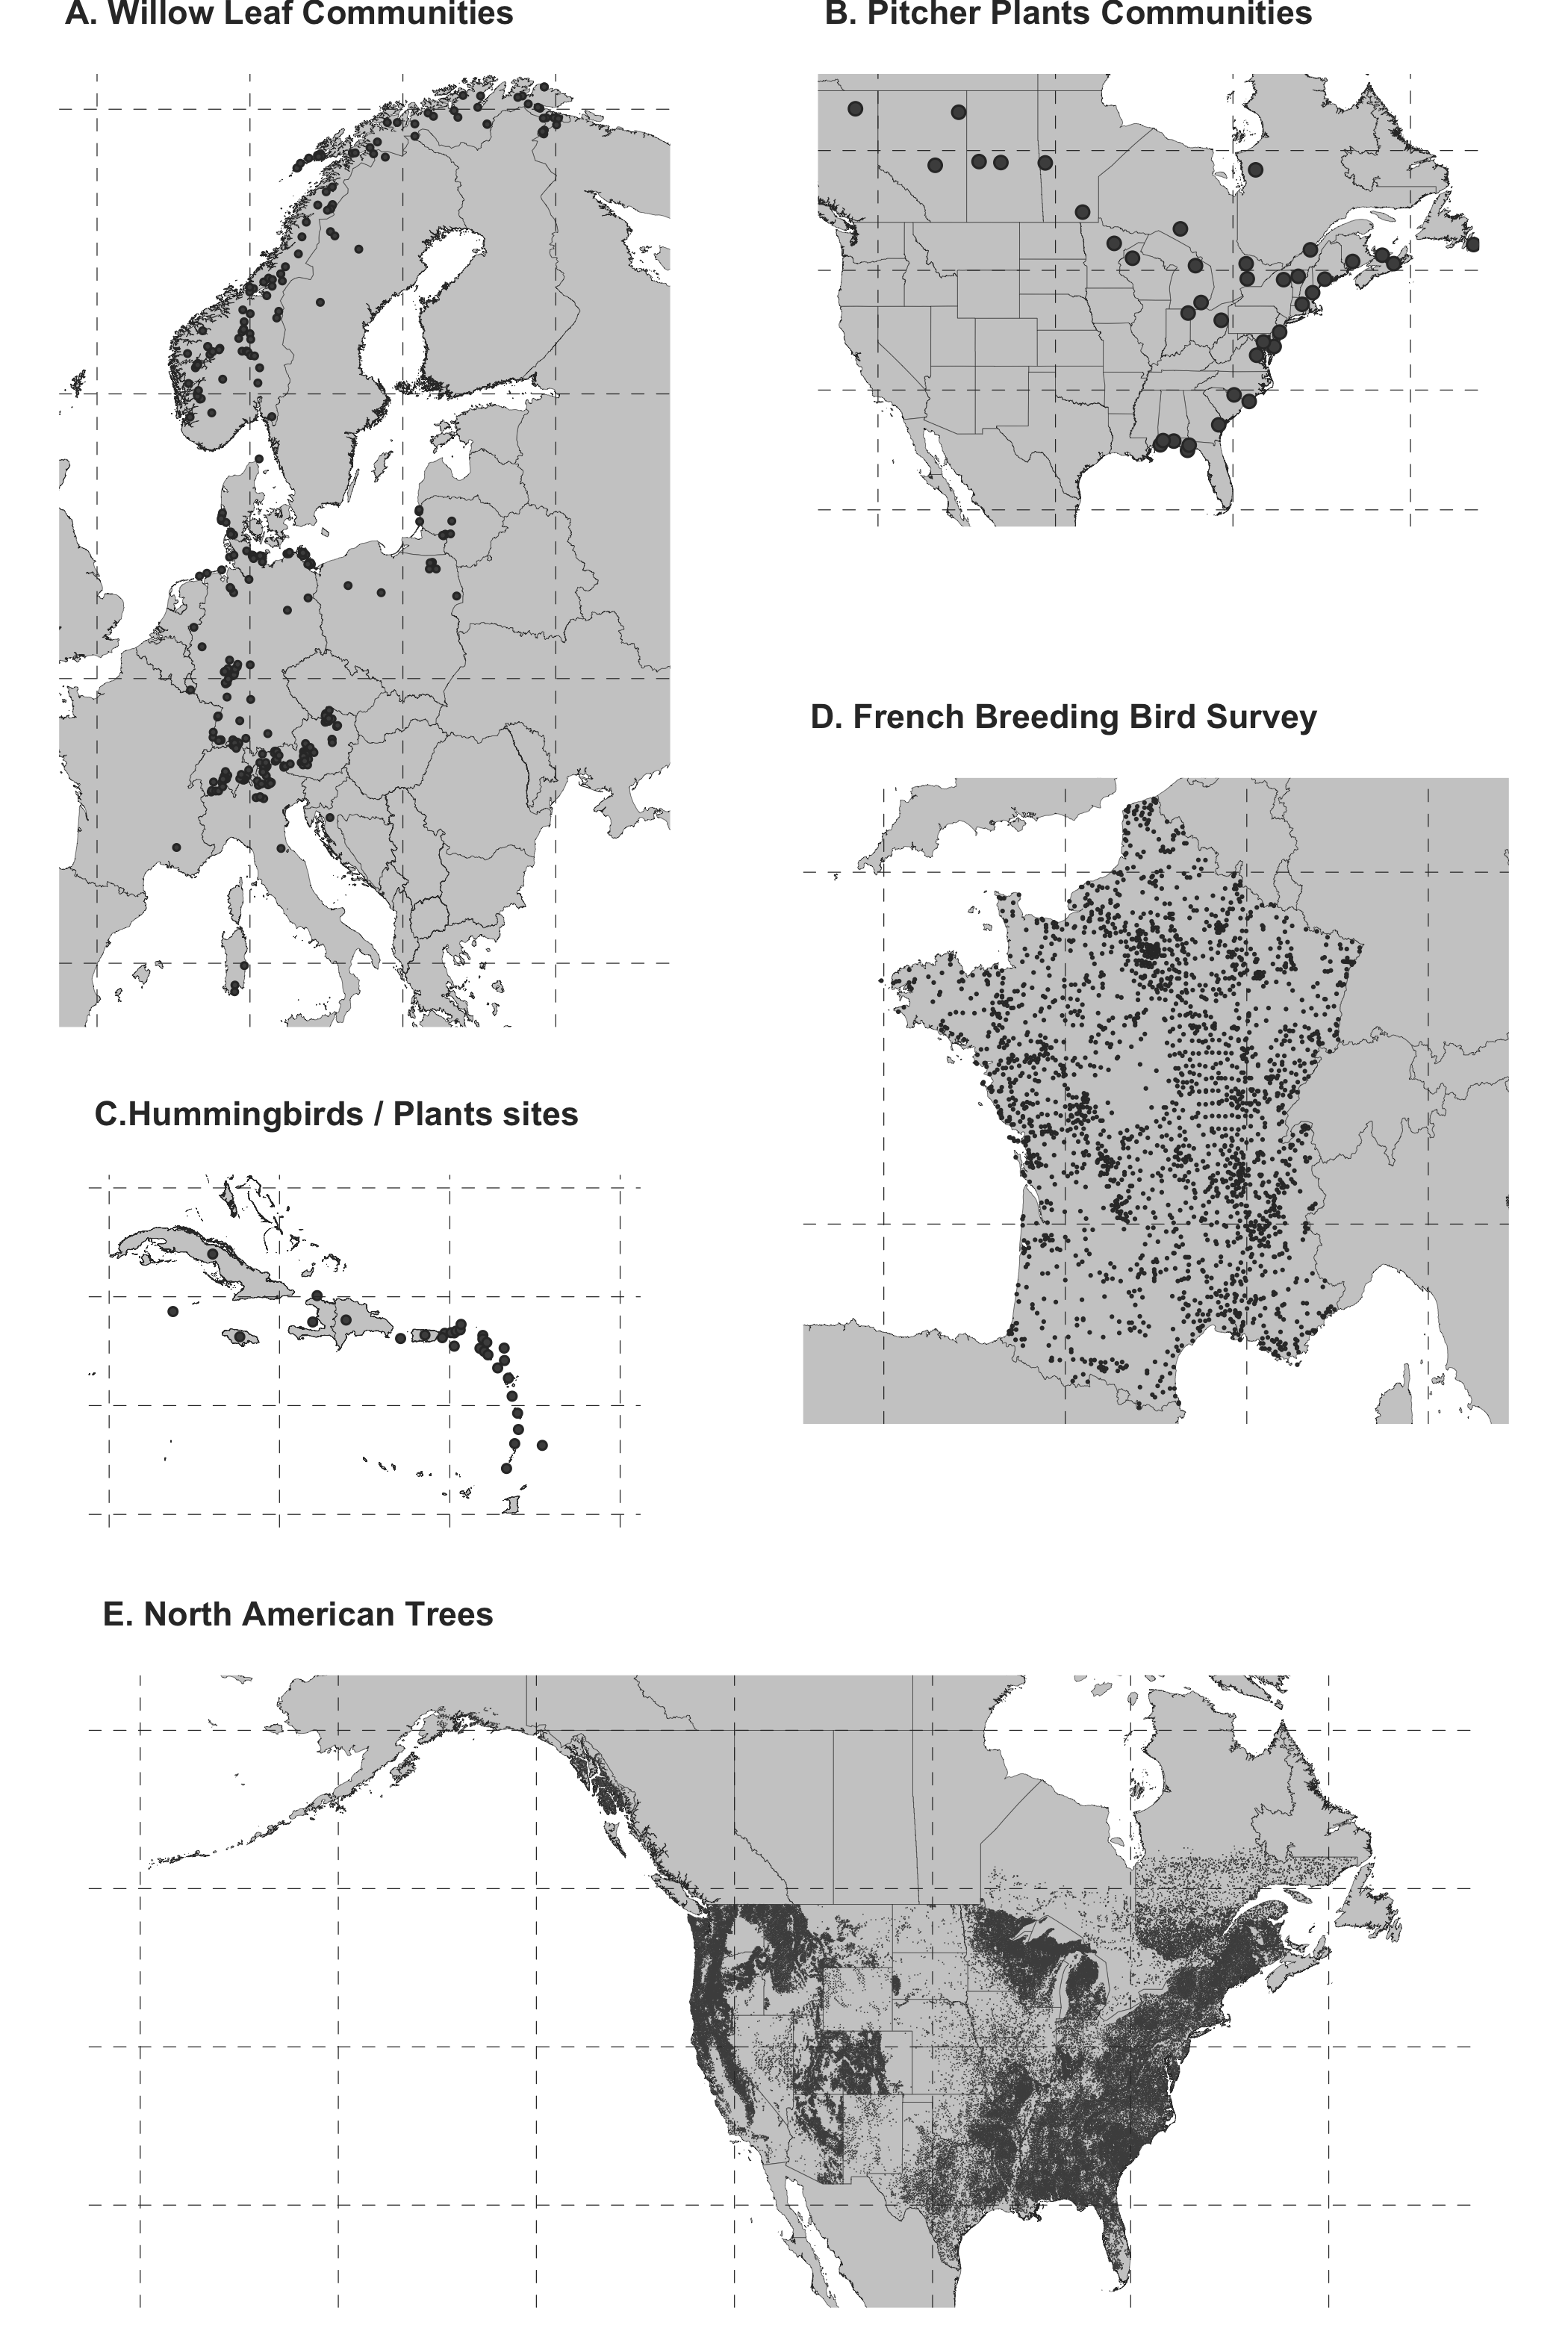
\includegraphics{../fig/figS1.png}
\caption{\textbf{Sites of the study}\label{fig:maps}}
\end{figure}

\newpage

\begin{figure}[htbp]
\centering
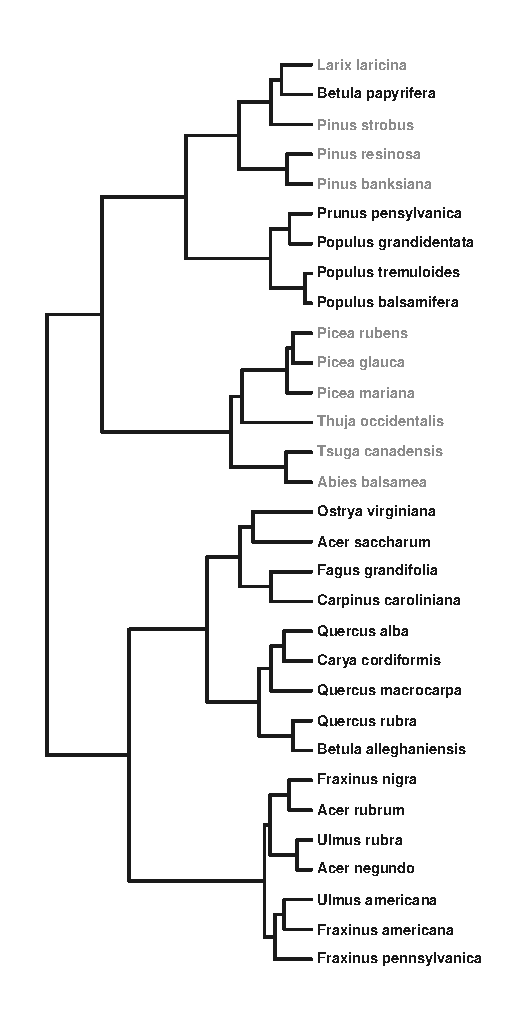
\includegraphics{../fig/figS2.pdf}
\caption{\textbf{Dendrogram representing the trait-based distances
between the 31 species studied in the North American tree datasets.}
Names of angiosperm species are written in dark grey while names of
Gymnosperm species are in a lighter grey.\label{fig:dendro}}
\end{figure}

\newpage

\begin{figure}[htbp]
\centering
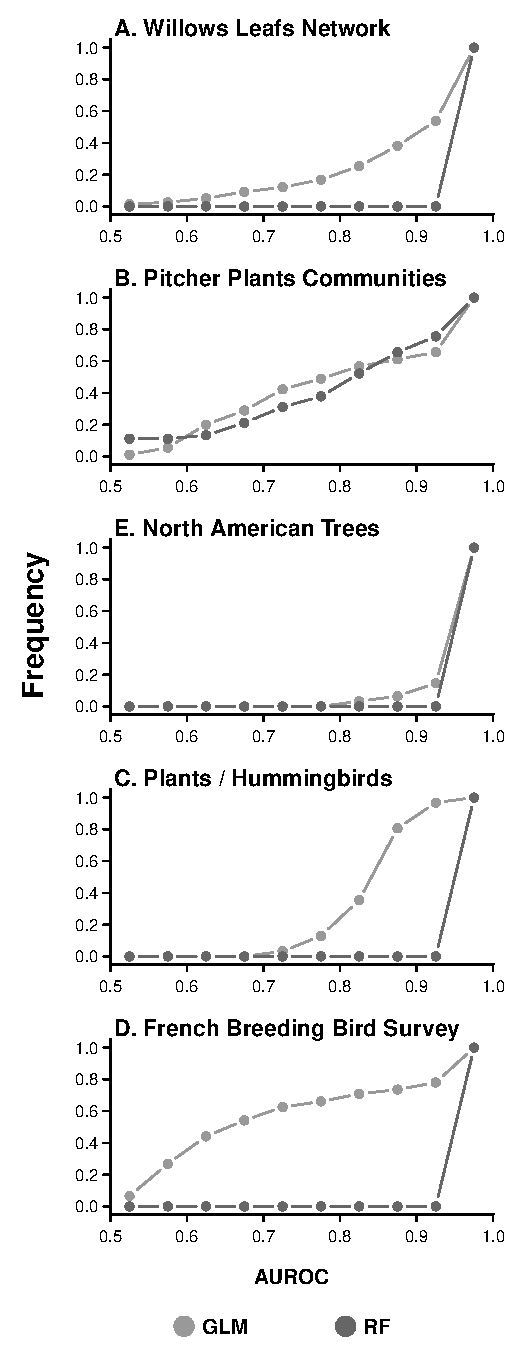
\includegraphics{../fig/figS3.pdf}
\caption{\textbf{Evaluation of the SDM approaches} For each dataset, the
distributions of performance of generalized linear models (light grey
symbols) and random Forest (dark grey symbols) for all species are
presented.\label{fig:auc}}
\end{figure}

\newpage

\begin{figure}[htbp]
\centering
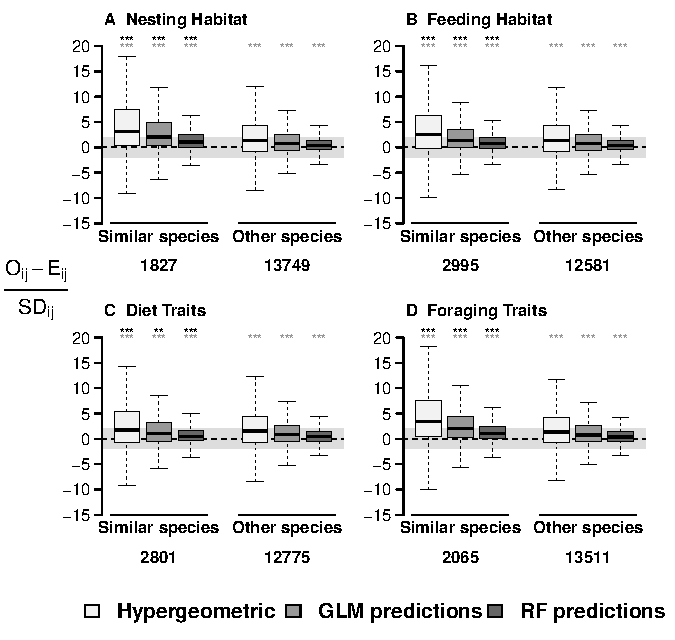
\includegraphics{../fig/figS4.pdf}
\caption{** Co-occurrence and the nature of the trait-based distance in
the FBBS dataset** The different panels correspond to four different set
of trait upon which for different distance are built. Similar species
are defined as the species for which the trait-based distance is less
than or equal to the lower decile of this distance distribution. Note
that outliers are not displayed. The light grey rectangle corresponds to
the 95\% confidence interval for the standard normal distribution which
gives insight into the proportion of pairs of species significantly
different from 0. P values were computed using the Wilcoxon rank sum
test, to compare interacting versus not-interacting Z-score distribution
calculated for the three different methods (black symbols) and to show
whether whether Z-score were greater for hypergeometric versus GLM and
whether GLM versus RF (grey symbols).}\label{figdist}
\end{figure}

\newpage

\begin{figure}[htbp]
\centering
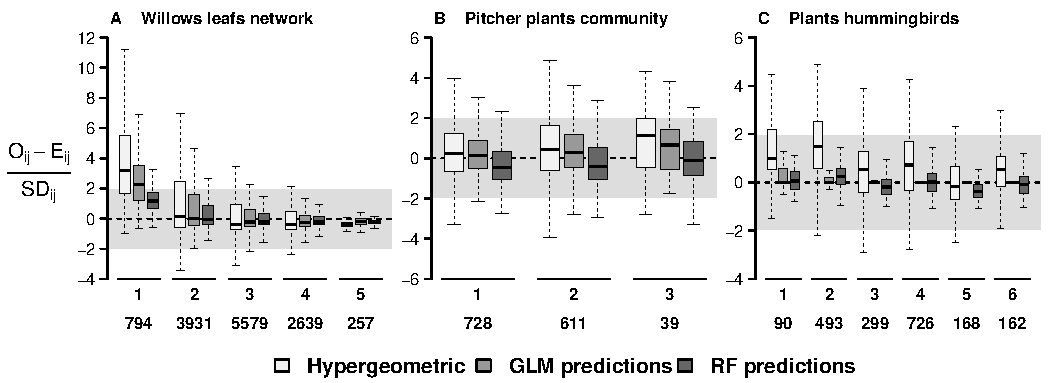
\includegraphics{../fig/figS5.pdf}
\caption{\textbf{Co-occurrence signal decays when the shortest path
between a pair of species decay} Distribution of Z-scores for all
interactions are grouped by shortest-path indicated by the first numbers
below boxplots. The other figures below stand for the number of pairs of
species included within the distributions.\label{fig:sht_pth2}}
\end{figure}

\newpage

\begin{figure}[htbp]
\centering
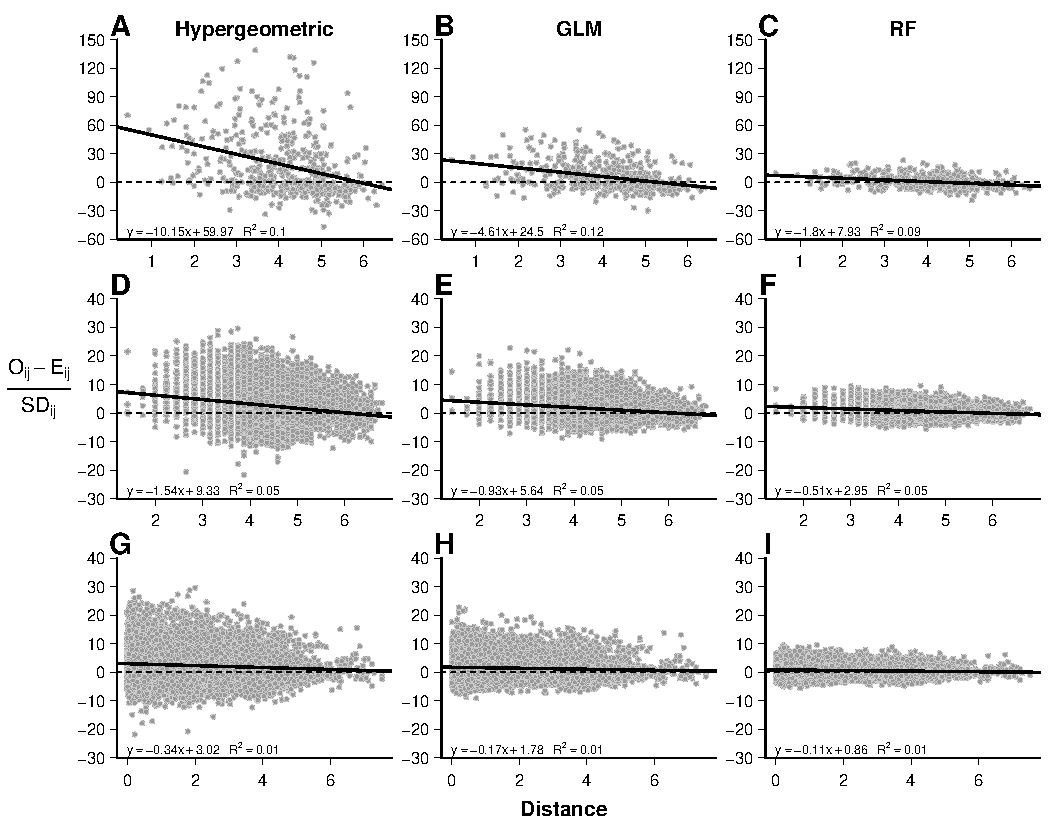
\includegraphics{../fig/figS6.pdf}
\caption{\emph{Changes co-occurrence signal when increasing the distance
between two species} Points represent the result for all pairs of
interaction for two datasets: the North American Tree dataset (A=C) and
the FBBS (D-I). For the latter, we used the trait-based distance
computed with all available traits (D-F) and the body-size ratios (the
lighter species over the heavier, panels G-I). In each panel, the
equation on the bottom-left corner indicated the results of the linear
regression depicted by the dotted line.\label{fig:distrev}}
\end{figure}

\newpage

\begin{figure}[htbp]
\centering
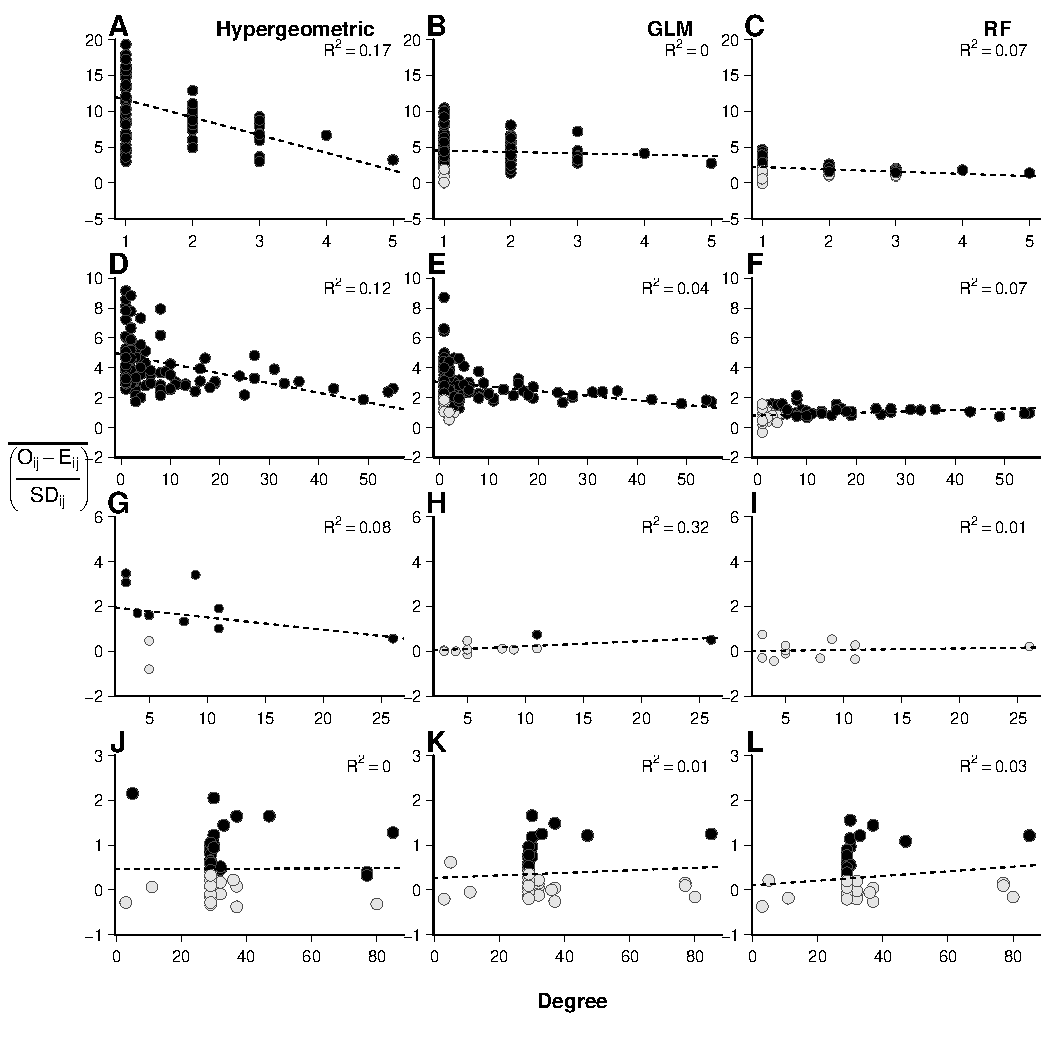
\includegraphics{../fig/figS7.pdf}
\caption{\textbf{The degree of species partially explains the decrease
of the co-occurrence strength} For the herbivores (A-C) and the
parasitoids in the willow leafs network datasets (D-F), the hummingbirds
in the Caribbean hummingbirds datasets (G-I) and all species in the
pitcher plants network that consume other species (J-L) the mean Z-score
is plotted against the degree of the species. Black symbols are mean
Z-scores significantly different from 0 (see SI Text). In each panel,
the dotted line represents the linear regression \(y~ax+b\) for which
the \(R^2\) is provided.\label{fig:degree}}
\end{figure}

\newpage

\begin{figure}[htbp]
\centering
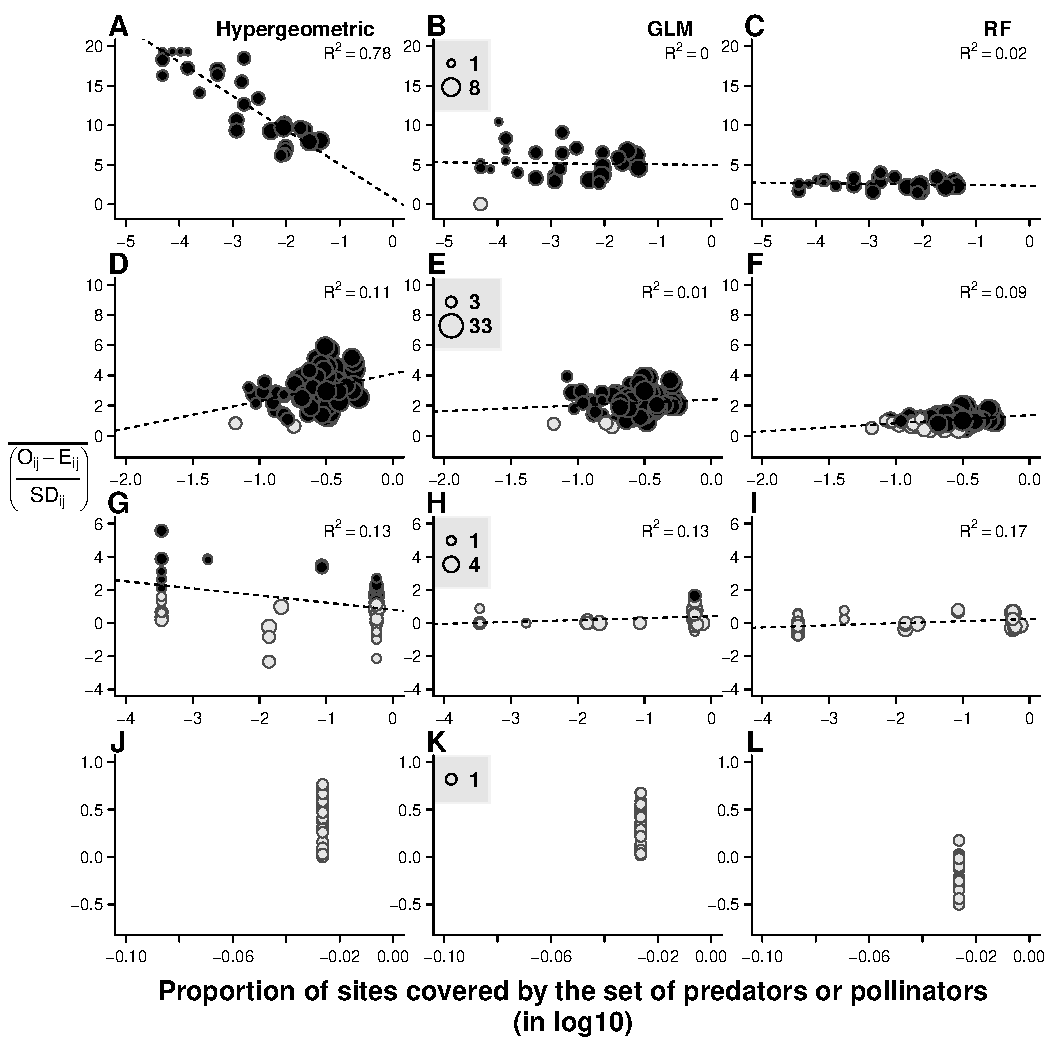
\includegraphics{../fig/figS8.pdf}
\caption{*Reversed figure 4** This figures correspond to the figure 4 in
the main text but the Z-score are calculated for preys (host plants)
rather than for predators 9pollinators). Mean Z-score are computed for
willows (A-C) and herbivores (based on the herbivores-parasitoids only,
D-F) of the willows leafs network, the hosts plants in the Caribbean
hummingbirds datasets (G-I) and species that feed on the detritus in the
pitcher plants network (panels J-L). The x-axis is expressed as a log
proportion of the total number of sites included in the considered
dataset. Black symbols are mean Z-scores significantly different from 0
(see SI Text). In each panel, the dotted line represents the linear
regression \(y~ax+b\) for which the \(R^2\) is provided. The size of
circles reflects the degree of species for which the Z-score was
calculated, the relation size-degree for each row is given in the middle
panel.\label{fig:degocc2}}
\end{figure}

\newpage

\begin{figure}[htbp]
\centering
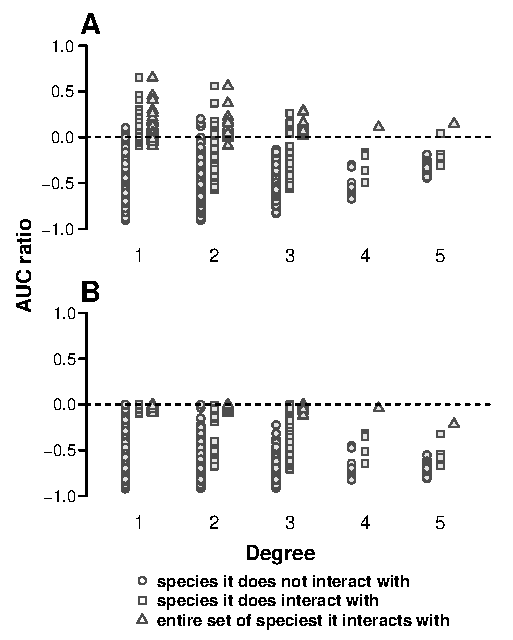
\includegraphics{../fig/figS9.pdf}
\caption{\textbf{Predicting herbivore distribution based on the
distribution of willows} For the herbivores in the willow leafs network
dataset, we compared the AUC obtained when using willow it does not
interact with (circles) a willow in interacts with (squares) and the set
of willow it interacts with (triangles) to AUC obtained for GLM (A) and
RF (B). Positive values indicated that species based model outperformed
the SDM model.\label{fig:ratauc}}
\end{figure}

\newpage

\newpage

\section*{Supporting References}\label{supporting-references}
\addcontentsline{toc}{section}{Supporting References}

\hypertarget{refs}{}
\hypertarget{ref-Dray2007}{}
Dray, S., Dufour, A.B., 2007. The ade4 Package: Implementing the Duality
Diagram for Ecologists. Journal of Statistical Software 22, 1--20.
doi:\href{https://doi.org/10.1.1.177.8850}{10.1.1.177.8850}

\hypertarget{ref-Rcoreteam2015}{}
R Core Team, 2015. R: A Language and Environment for Statistical
Computing.

\hypertarget{ref-Veech2013}{}
Veech, J.A., 2013. A probabilistic model for analysing species
co-occurrence. Global Ecology and Biogeography 22, 252--260.
doi:\href{https://doi.org/10.1111/j.1466-8238.2012.00789.x}{10.1111/j.1466-8238.2012.00789.x}
